\documentclass[10pt,oneside,a4paper]{article}
\usepackage{amsmath}
\usepackage{amsfonts}
\usepackage{amssymb}
\usepackage{fancyhdr}
\usepackage[bottom=0.5in]{geometry}
\usepackage{graphicx}
\usepackage{float}
\usepackage{hyperref}
\usepackage{xcolor}
\pagestyle{fancy}
\topmargin -0.5in
\lhead{BioE Methods Lab}
\chead{Myoelectric Tetris}
\rhead{Bioelectric Signals}
\begin{document}
\section{Introduction}
Researchers are currently working on ways to control devices using bioelectric signals. In this portion of the lab you will build an EMG signal classifier to implement myoeletric, or muscle, control in a game of Tetris in Matlab. 
\section{Software Setup}
Streaming data from SpikerBox into Matlab requires a separate USB interfacing library that is implemented in Python. To get data in real time from SpikerBox, you will need to install Python and the Python USB library \texttt{hidapi}. The next several sections take you through how to install Python and the \texttt{hidapi} library.
\subsection{Installation on Windows}
Matlab Tetris requires Python to be installed to interface with the USB. This section walks through how to install Python, \texttt{pip}, and \texttt{hidapi}. If you already have any of these installed, jump to the appropriate section.
\subsubsection{Install Python}
To install Python, download the \href{https://www.python.org/ftp/python/3.6.4/python-3.6.4-amd64.exe}{\color{blue}Python installer} from Windows if you have a 64-bit computer. On the first screen, make sure to check the box that reads ``Add Python 3.6 to PATH''. Select ``Install Now'' and click ``Yes'' if your computer asks for administrator privileges: 
\begin{figure}[H]
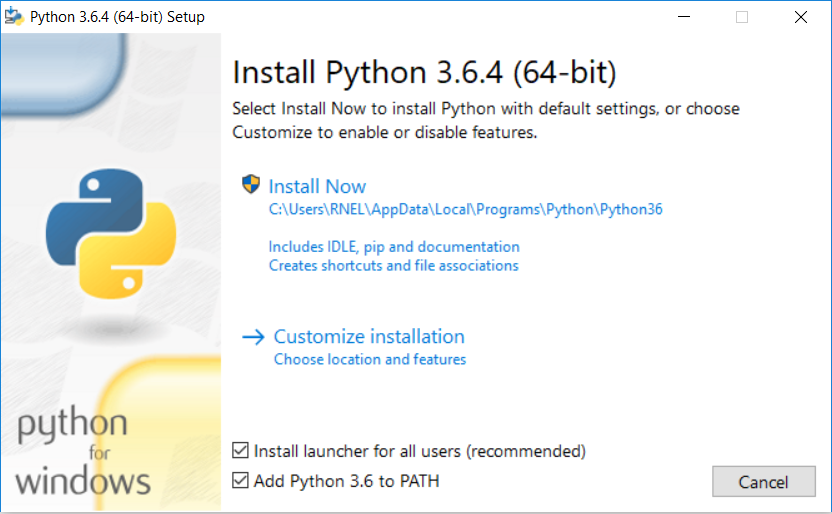
\includegraphics[width=\textwidth]{image.png}
\end{figure}
Once installation has completed, open ``Command Prompt'' in your start menu and ensure that Python is installed by typing \texttt{python} into the command line and pressing enter. If you see ``Python 3.6.4'' and other details, then Python has been correctly installed:
\begin{figure}[H]
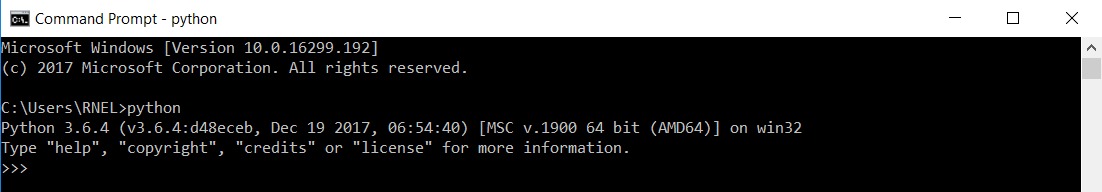
\includegraphics[width=\textwidth]{commandline.png}
\end{figure}
\subsubsection{Install \texttt{pip}}
Install \texttt{pip} by downloading the \href{https://bootstrap.pypa.io/get-pip.py}{\color{blue}script} \textbf{into your user directory} \texttt{(C:\textbackslash Users\textbackslash <USER>)}. Exit the Python shell in the command line by typing \texttt{exit()} and install \texttt{pip} with the command:
\begin{verbatim}
python get-pip.py
\end{verbatim}
\begin{figure}[H]
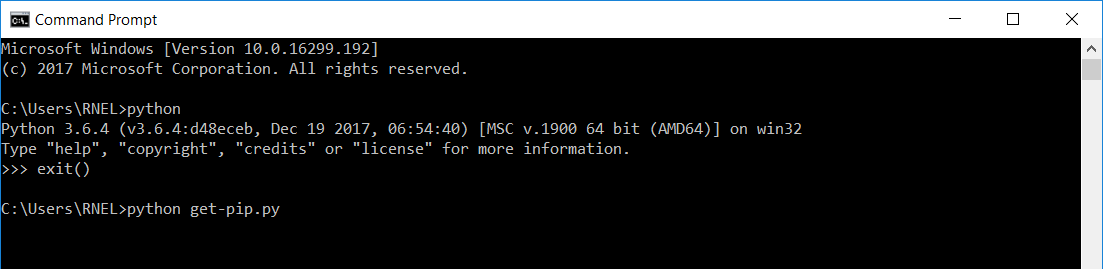
\includegraphics[width=\textwidth]{pip.png}
\end{figure}
Verify that \texttt{pip} is installed by typing \texttt{pip -version} into the command line and pressing \texttt{Enter}:
\begin{verbatim}
C:\Users\RNEL>pip -version
\end{verbatim}
You should see a similar output:
\begin{verbatim}
pip 9.0.1 from c:\users\rnel\appdata\local\programs\python\python36\lib\site-packages
\end{verbatim}
This means that \texttt{pip} has been successfully installed.
\subsubsection{Install \texttt{hidapi}}
The easiest way to install \texttt{hidapi} is through \texttt{pip} on Windows. In the command prompt, install  \texttt{hidapi} with the following command and press enter:
\begin{verbatim}
C:\Users\RNEL>pip install hidapi
\end{verbatim}
A quick way (optional) way to test your \texttt{hidapi} install is to run the following commands:
\begin{verbatim}
C:\Users\RNEL>python
\end{verbatim}
Then, in the Python shell, try:
\begin{verbatim}
>>> import hid
\end{verbatim}
If the import succeeds, \texttt{hidapi} has been successfully installed.
\subsection{Download Myoelectric Tetris}
Download the code for \href{https://github.com/mfliu/Myoeletric_Tetris} {\color{blue} Myoelectric Tetris} by downloading the \texttt{.zip} file and unzipping it into a directory of your choice. In the directory, there should be the following files: \\
\begin{enumerate}
\item \texttt{emg\_buffer.py}: This is the Python script that gets EMG data from SpikerBox. \textbf{Do not change this file}.
\item \texttt{py\_emg\_buffer.m}: The Matlab connector to \texttt{emg\_buffer.py}. \textbf{Do not change this file either.}
\item \texttt{test\_emg\_buffer.py}: A simple Python script to test the USB interface manager implemented in \texttt{emg\_buffer.py}. Running this in a Python shell allows for debugging of the Python USB library, but should not be necessary for this portion of the lab.
\item \texttt{matlabtetris.m}: The main function that runs Tetris in Matlab, reads EMG data from SpikerBox, and calls the EMG classification function that you write. Run this function to start a game of Tetris.
\item \texttt{set\_window\_size.m}: Set the time window of EMG to buffer for classification, in milliseconds. 
\item \texttt{emg\_control.m}: The EMG signal classifier. This Matlab script takes in two channels of raw EMG input and outputs an array of length 3 corresponding to the direction the Tetris piece should move (left, right, or turn).
\end{enumerate}
\section{Implementing Myoelectric Control}
In this portion of the lab, you will be adjusting settings on a root-mean-square-based EMG classifier to control pieces in a game of Tetris. Hook up the SpikerBox to electrodes on a forearm flexor-extensor muscle pair and turn SpikerBox on. Try running \texttt{matlabtetris.m}. You should see the Tetris game pop up in a new window. Press \texttt{Start}. The game should begin, and you will see a scatter plot of RMS values from each EMG channel.
\begin{figure}[H]
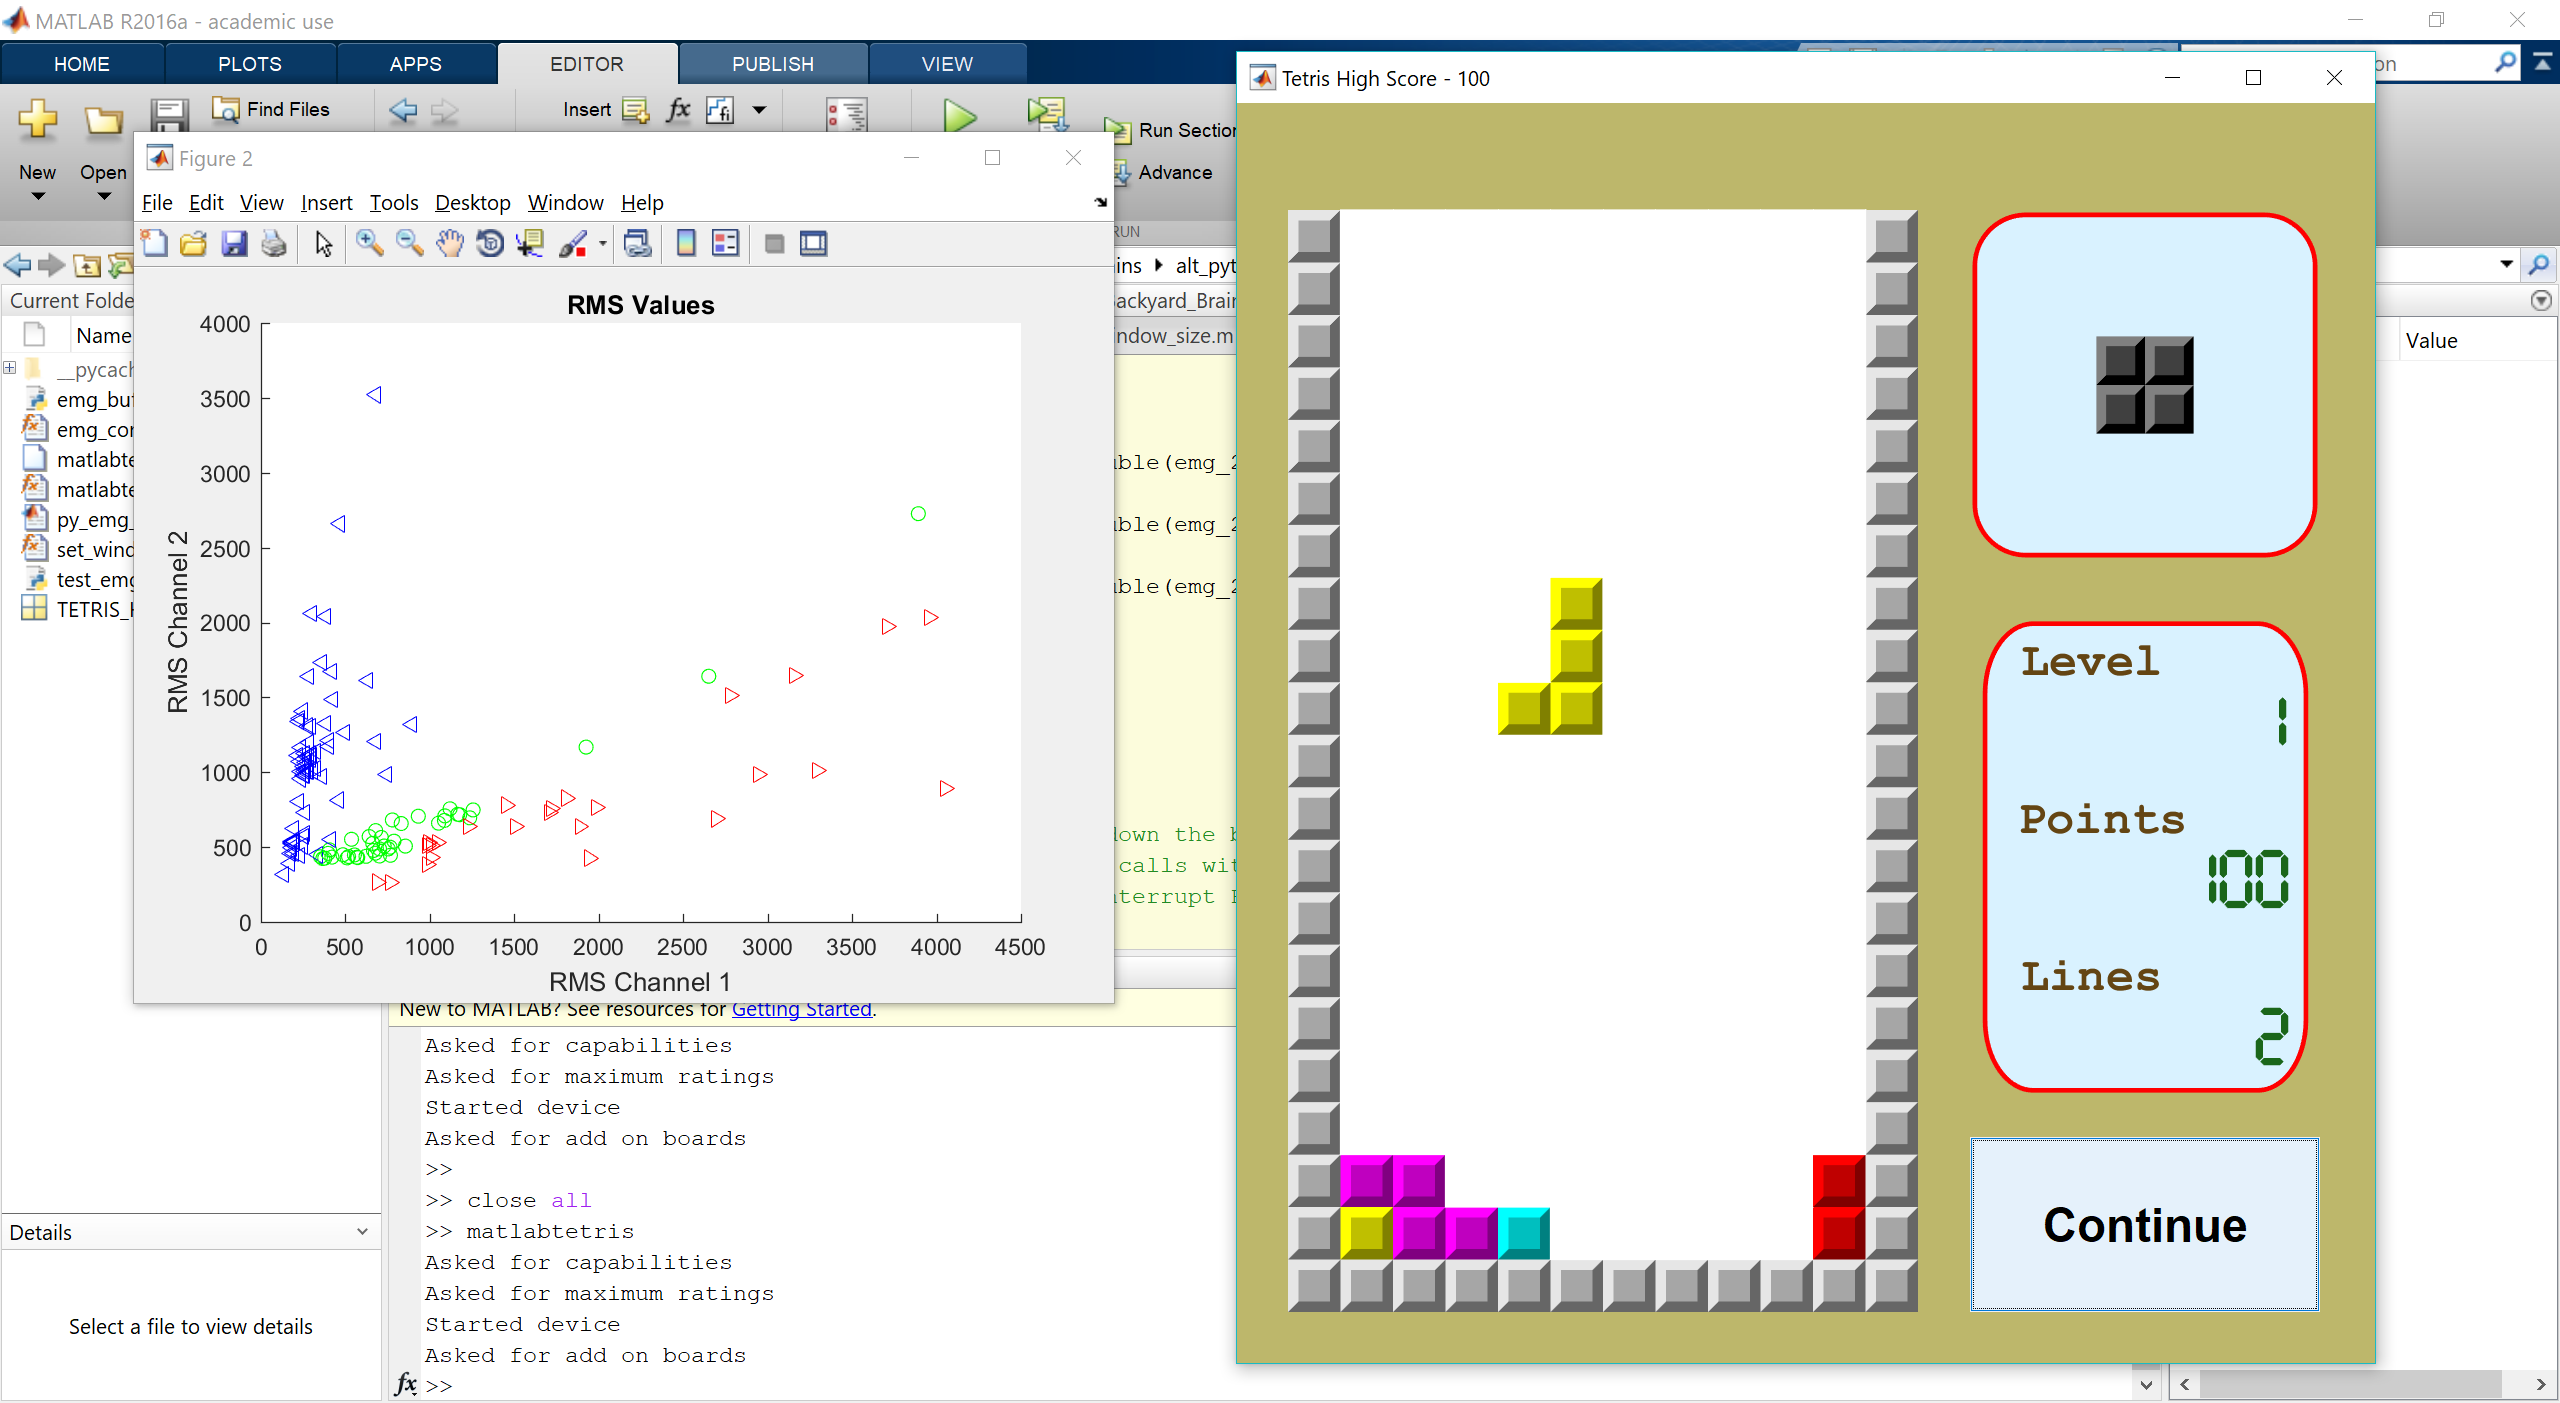
\includegraphics[width=\textwidth]{tetris_game.PNG}
\end{figure}
\subsection{RMS Classification}
Open \texttt{emg\_control.m}. This Matlab function is where the classifier is implemented. It takes as input the raw signal of two EMG recording channels, which provide signal from your wrist flexor muscle and wrist extensor muscle. Using these raw EMG signals, \texttt{emg\_control.m} computes the RMS of the signal on each channel and performs a simple thresholding based on the ratio of the RMS of the two channels. The function returns an array of length 3, where a value of 1 in the first element means the Tetris piece should move left, a value of 1 in the second element means the piece should move to the right, and a value of 1 in the last element indicates the Tetris piece should turn in the clockwise direction. Since the Tetris piece can only make one movement per timestep, only one element in the vector is nonzero. This is called a \textbf{one-hot encoding} scheme. 
\begin{verbatim}
function [left, right, turn] = emg_control(emg_1, emg_2)
left = 0;
right = 0;
turn = 0;

rms_1 = rms(emg_1);
rms_2 = rms(emg_2);
\end{verbatim}
 
Currently, the classifier is a rough threshold on the ratio of RMS of channel 1 to RMS of channel 2. Think about how you should set the thresholds on the RMS ratio based on which muscles your electrodes are hooked up to. For example, if channel 1 is recording the wrist flexors in your forearm, then a RMS ratio $\frac{RMS(Channel1)}{RMS(Channel2)} > 1$ would indicate that the wrist flexor muscles are contracting more strongly than the extensor muscles, so the piece should move to the left. Similarly, if the RMS ratio $\frac{RMS(Channel1}{RMS(Channel2)} = 1$, then your flexors and extensors are co-contracting approximately equally, which would mean you should turn your Tetris piece. 
\begin{verbatim}
if rms_1/rms_2 > 1.8
    right = 1;
elseif rms_1/rms_2 < 0.8
    left = 1;
elseif rms_1/rms_2 > 0.8 && rms_1/rms_2 < 1.8
    turn = 1;
end
\end{verbatim}
Think about what thresholds or aspects of the EMG signal you would want to use for classification. The scatter plot of RMS values of each channel may help you.

The scatter plot in the figure above shows the classification of each point. As you classify EMG signals during the game, a point corresponding to (RMS(Channel1), RMS(Channel2)) will be plotted in the scatter plot with the color and shape indicating what your classifier labeled that point as. {\color{blue} Blue arrows} pointing left indicate that the classifier predicted that the Tetris piece should move left, {\color{red} red arrows} pointing right indicate the Tetris piece moved right, and {\color{green} green circles} indicate that the Tetris piece rotated.

Try playing Tetris a couple times and look at where the RMS values fall. Move the Tetris piece with some flexion, extension, and co-contraction movements. If your electrodes are on your left arm, then a wrist flexion indicates that the Tetris piece should move to the right. Look at where the point shows up--does the classifier indeed plot a red rightward arrow for that point? Try a couple of other movements. Where do these points fall? Are there decision boundaries you can draw in this two-dimensional RMS space that will help you classify the movement the Tetris piece should do? Change the \texttt{if} statements in \texttt{emg\_control.m} to RMS ratios or threshold values that you think will classify the EMG signal the best.
\subsection{EMG Window Size}
Another factor in classification accuracy is the time window of EMG signal that we use. In \texttt{set\_window\_size.m}, set the length of the EMG signal (in milliseconds) you want to use for classification. Try different values ranging from 5ms to 500ms. What are the advantages of using a shorter time window? A longer time window?
\begin{verbatim}
function window_size = set_window_size()
window_size = 100; % in ms
end
\end{verbatim}
\section{Other Biosignal Controls}
In this lab, you studied how muscle activity can be used to implement myoelectric control in a Tetris game. How might other biosignals, such as eye movements, be used for control? What would your classification features be in that case?
\end{document}